\chapter{Element of Room Acoustics}\label{chap:acoustics}

\newthought{Synopsis} This chapter will cross an important bridges: from the physics to analog signal processing
Acoustics is basically how sounds works in environment.


\section{Sound Wave Propagation}\label{ch:acoustics:sec:wave}

Sound is a complex concept and complex concepts creates theories.


from https://plato.stanford.edu/entries/sounds/
The main relevant families of answers include proximal, medial, distal, and aspatial theories.
Proximal theories would claim that sounds are where the hearer is.
Medial theories—exemplified by mainstream acoustics—locate sounds in the medium between the resonating object and the hearer.
Distal theories consider sounds to be located at the resonating object. Finally, aspatial theories deny spatial relevance to sounds.

What is the definition? The etymology?
How is it perceived, how is it measured? How is it represented?

speed of sound

\begin{equation}
    \cair =  331.4 + 0.6\temperature + 0.0124\rhumidity \; \text{m/s}
    .
\end{equation}


If we think at the process of sound production in the light of the classic \textit{source-medium-receiver} model of communication theory,
we can say that in we have studied models for the source of sound signals. We now move a step further and examine the effects of the medium in which sound propagates, and the receiver, specifically a human receiver with two ears.

Equation are reproduced or modified from \cite{Kuttruff2009room, Marczuk2006modelling, Habets2010generator, Avanzini2019Chapter4, Allen1999image}

When vibrating objects excites air, molecules that start oscillating creating local pressure deviation from the atmospheric pressure.
Such vibration of of air molecules takes place in the direction of the excitement, with the next layer of molecules excited by the first layer.
The molecules oscillate in the frequency of the initial exciting vibration, creating oscillating of higher and lower density of molecules.
Pushing layer by layer forward, a \textit{longitudinal} wave is created.
% \marginpar{%
    % \animategraphics[loop,autoplay]{12}{./figures/general/Lwave-}{0}{50}
% }

Sound is mechanical energy in the form of pressure variances in an elastic medium. These pressure variances propagate as waves from a vibrating source.

Changes in air pressure (air being a propagating medium) can be represented by a WAVEFORM, which is a graphic representation of a sound. In reality, sound waves propagate through the air in LONGITITUDAL WAVES (and not TRANSVERSE WAVES):

\subsection{The Acoustic wave equation}
\label{subsec:acoustics:waveq}

The \textit{acoustic wave equation} governs the propagation of acoustic waves through a perfectly elastic medium (gas or liquid) in a 3D space.
The equation describes the evolution of acoustic pressure $\pressure$ as function of the position $\positionSource$ $[\si{\metre}]$ and time $t$ $[\si{\second}]$
\marginpar{%
    The symbol $\knabla^2 = \kpderiv[2]{}{x} + \kpderiv[2]{}{y} + \kpderiv[2]{}{z}$
    stands for the 3-dimensional \textit{Laplacian} operator.
}
\begin{equation}
    \label{eq:acoustics:wave}
    \knabla^2 \pressureSpaceTime - \frac{1}{\speedOfSound^2} \kpderiv[2]{\pressureSpaceTime}{t} = 0
    .
\end{equation}
The constant $\speedOfSound$ is the sound velocity in the medium with dimension $\frac{\si{\metre}}{\si{\second}}$.

As opposed to mechanical vibrations in a string or (drum) membrane, acoustic vibrations are \textit{longitudinal} rather than \textit{transversal},
\ie/ the air particles are displaced in the same direction of the wave propagation.
\marginpar{%
    In 1746, d’Alembert discovered the one-dimensional wave equation for music strings,
    and within ten years Euler discovered the three-dimensional wave equation for fluids.
}

Assuming the propagation of the wave in a homogeneous medium, one can obtain the equation above by combining three fundamental physical laws:
\begin{itemize}
    \item the \textit{conservation of momentum}\sidenote{its appliction to fluids comes with the name of the Euler's equation},
    \item the \textit{conservation of mass} (\aka/ the continuity equation), and
    \item the \textit{equation of state} (\aka/ the gas law)
\end{itemize}
In case of inhomogeneous medium, scalar inhomogeneities, \eg/ due to temperature variation,
and vector inhomogeneities, \eg/ due to presence of fans or air conditioning
brakes the underlying assumption of the model.
However these effect are typically small in typical application of speech and audio signal processing.
Thus they are commonly ignored.

\newthought{The Derivation of}~\cref{eq:acoustics:wave} starts by considers a infinitesimal volume unit $V$ of a fluid or gas (such as air), whose center of gravity is located at $\positionMicrophone$.
Let $\mass$ be the mass of such volume.
By the well-known Newton's second law, applying a force $F$ to the fluid, its acceleration increase proportionally to $\mass$,
namely:
\begin{equation}
    \label{eq:acoustics:newton}
    \forceVec = \mass \kpderiv[]{\velocity\depSpaceTime}{t}
\end{equation}
\marginpar{%
Newton's Law II: The alteration of motion is ever proportional to the motive force impress'd;
and is made in the direction of the right line in which that force is impress'd.
\\Orignal: \emph{Lex II: Mutationem motus proportionalem esse vi motrici impressae,
et fieri secundum lineam rectam qua vis illa imprimitur.}
}
where $\velocity(\positionSource, t)$ denotes the volume velocity and $t$ the time $[\si{\second}]$.
The force can be expressed in terms of difference of acoustic pressure $p$ at $\positionMicrophone$ on a surface of the volume, $\surface$, namely
\begin{equation}
    \label{eq:acoustics:pressure}
    \forceVec = - V \kbracket{\kgrad{\pressureSpaceTime}}
\end{equation}
where $\kgrad{}$ is is the gradient operator.
By combining \cref{eq:acoustics:newton,eq:acoustics:pressure}, we obtain the famous \textit{Euler's equation of motion}:
\begin{equation}
    \label{eq:acoustics:euler}
    \kgrad{\pressureSpaceTime} = - \densityEq \kpderiv[]{\velocity\depSpaceTime}{t}
\end{equation}
where $\densityEq = \frac{\mass}{\surface}$ is the static density of the medium
\footnote{%
\label{fn:acoustics:airconstanc}
\\Air Denisity $\density_{\text{air}} = 1.18 \tfrac{\si{\kilogram}}{\si{\metre^3}}$.
\\Air Gas constant $R_{\text{air}} = 286.9 \tfrac{\si{\joule}}{\si{\kilogram} \si{\mole}}$.
\\Air Adiabatic index $\gamma_{\text{air}} = 1.4$.
\\Speed of sound in air $\speedOfSound_{\text{air}} = 343.1 \tfrac{\si{\metre}}{\si{\second}}$.
}.

\newthought{Secondly, by the Conservation of Mass} principle,
the total mass must remain constant as the it is in a deformable medium. This principle
translates into the \textit{continuity equation}, written in the differential form:
\begin{equation}
    \label{eq:acoustics:continuity}
    \kpderiv[]{\eta\depSpaceTime}{t} = V \kbracket{\divergence{\bfq\depSpaceTime}}
\end{equation}
where
\begin{itemize}
    \item $\eta\depSpaceTime$ is the the amount of the quantity q per unit volume
    \item $\eta\depSpaceTime$ is the volume variation due to the pressure changing
\end{itemize}
inside the volume $\volumeUnit$ in time is equal to the total amount of mass passing thought the surface .

\newthought{Finally, the State Equation} describes the properties of the propagation medium.
Assuming that the fluid (or gas) to be ideal, the \textit{Charles-Boyle} gas law states\sidenote{The original gas law writes $P V = n R T$. Here the law is written in terms of \textit{specific volume}}
\begin{equation}
    P V = R T
\end{equation}
where $P$ is the total pressure on the volume $V$; $T$ the absolute temperature in degrees Kelvin and $R$ is specific gas constant\cref{fn:acoustics:airconstanc}.
The dependency upon space and time $\depSpaceTime$ is here omitted for sake of compactness and readability.

Since the exchange of heat of wave of acoustic frequencies range in negligible, the whole process can be considered thermodynamically \textit{adiabatic}.
In such scenario, the relation between the total pressure and the volume is given by
\begin{equation}
    \label{eq:acoustics:state}
    P V^\gamma = \const
\end{equation}
where $\gamma$ is the adiabatic index of the medium~\cref{fn:acoustics:airconstanc}.

The total pressure and the total volume consist in a sum of a constant and a variable term, that is $P = P_0 + p$, $V = V_0 + \nu$ respectively.
Considering that $p \ll P_0$ and $\nu \ll V_0$, the time-differential of~\cref{eq:acoustics:state} with respect to time reads
\begin{equation}
    \label{eq:acoustics:statediff}
    \kpderiv[]{\pressureSpaceTime}{t} = - \gamma \frac{P_0}{V_0} \kpderiv[]{\nu\depSpaceTime}{t}
\end{equation}

\newthought{Finally, the Acoustic Wave Equation} can be now derived by combining together
the equation of motion~\ref{eq:acoustics:euler},
the continuity equation~\ref{eq:acoustics:continuity},
and the state equation~\ref{eq:acoustics:statediff}.
In particular the combination of~\cref{eq:acoustics:continuity,eq:acoustics:statediff},
\begin{equation}
    \kpderiv[]{\pressureSpaceTime}{t} = - \gamma P_0 \kbracket{\divergence{\bfq\depSpaceTime}}
    ,
\end{equation}
can be differentiated with respect to time $t$ yielding to
\begin{equation}
    \kpderiv[2]{\pressureSpaceTime}{t} = - \gamma P_0 \kbracket{\divergence{\kpderiv[]{\bfq\depSpaceTime}{t}}}
    .
\end{equation}
Taking the divergence of each side of the~\cref{eq:acoustics:euler}, we get
\marginpar{%
The \textit{Laplacian} of a function is the given by the divergence of the gradient of that function,
\\in math $\knabla^2 x = \divergence{\kgrad{x}}$}
\begin{equation}
    \knabla^2 \pressureSpaceTime = -\densityEq \kbracket{\divergence{q\depSpaceTime}}
\end{equation}
The above two equation can be combined leading to
\begin{equation}
    \knabla^2 \pressureSpaceTime = \frac{1}{\speedOfSound^2} \kpderiv[2]{\pressureSpaceTime}{t}
\end{equation}
where the $\speedOfSound$ is the speed of sound and is related to the medium properties through
\begin{equation}
    \speedOfSound^2 = \frac{\gamma P_0}{\densityEq}
    .
\end{equation}


\newthoughtpar{The Helmholtz's equation}
The wave equation~\ref{eq:acoustics:wave} is expressed in the space-time domain $\depSpaceTime$.
By applying the temporal Fourier transform to the wave equation we obtain the time-independent \textit{Helmholtz equation} is obtained, \ie/
\begin{equation}
    \label{eq:acoustics:helmholtz}
    \knabla^2 P(\positionMicrophone, f) + k^2 P(\positionMicrophone, f) = 0
    ,
\end{equation}
where $k \frac{2 \pi f}{c}$ denotes the \textit{wave number}, that relates the frequency $[\si{\hertz}]$ and the propagation velocity.

The wave equation~\ref{eq:acoustics:wave} and the Helmholtz's equation~\ref{eq:acoustics:helmholtz} are source independent,
namely no source is present in the medium. Therefore they called \textit{homogeneous} as the right-hand term are zero.

Normally the sound field is a complex field generated by multiple acoustics sources. As consequence, the two equation becames
inhomogeneous as some non-zero terms needs to be added to the right-hand sides.
\todo{cite [27]}

In presence of a sound source producing waves with distribution function $s(t, \positionSource)$, the wave equation can be written
\begin{equation}
    \label{eq:acoustics:source}
    \knabla^2 \pressureSpaceTime - \frac{1}{\speedOfSound^2} \kpderiv[2]{\pressureSpaceTime}{t} = s(t, \positionSource)
    .
\end{equation}
Then, the correspondent Helmholtz's equation writes
\begin{equation}
    \label{eq:acoustics:source_freq}
    \knabla^2 P(\positionMicrophone, f) + k^2 P(\positionMicrophone, f) = - S(\positionSource, f)
    .
\end{equation}

For instance one can assume an infinitesimally small pulsating sphere locate at $\positionSource$ radiating constant acoustic energy at frequency $f$.
For the receiver position $\positionMicrophone \neq \positionSource$, the Helmholtz's equation writes

\begin{equation}
    \label{eq:acoustics:green_definition}
    \knabla^2 H(f, \positionMicrophone \mid \positionSource)
     + k^2 H(f, \positionMicrophone \mid \positionSource) = - \delta(\positionMicrophone - \positionSource)
    ,
\end{equation}
where the term $H(f, \positionMicrophone \mid \positionSource)$ is an \textit{Green's function}.
For the properties of the Green's functions, $H(f, \positionMicrophone \mid \positionSource)$ is also solution of the homogeneous Helmholtz equation~\ref{eq:acoustics:helmholtz}.
The source is describe here by $\delta(\positionMicrophone - \positionSource)$, which in this context is a 3-dimension Dirac function.
We will see in the next subsection that the function $H$ solving~\ref{eq:acoustics:green_definition} can be interpreted as the free-field \textit{Transfer Function}
between the source at $\positionSource$ and the receiver at $\positionMicrophone$.

\subsection{... and its solution as Green's function}
\textsc{The Green's Functions} are mathematical tools for solving linear differential equations with specified initial- and boundary- condition \cite{Duffy2015}.
\marginpar{%
\footnotesize
By 1950 Green’s functions for Helmholtz’s equation were used to find the
wave motions due to flow over a mountain  and in acoustics.
Green’s functions for the wave equation lies with Gustav Robert Kirchhoff (1824–1887),
who used it during his study of the three-dimensional wave equation.
He used this solution to derive his famous \textit{Kirchhoff’s theorem}.
\\--- Duffy, 2015.
}
They have been used to solve many fundamentals equation, among which \cref{eq:acoustics:helmholtz,eq:acoustics:wave} for both free and indoor propagation.
They can be seen as the equivalent concept of the \textit{impulse responses} (\resp/ transfer function) used in signal processing.
Under this light and by assuming the fluid  medium as the \textit{linear filter}, the physic so-far can be rewritten in the vocabulary of
the communication theory, namely \textit{input}, \textit{filter} and \textit{output}.

Green say that the partial differential equations above can be solved for arbitrary source as follows:

\begin{equation}
    \label{eq:acoustics:helmholz_conv}
    P(f, \positionMicrophone) = \iiint_{\volume_\contSource} H(f, \positionMicrophone \mid \positionSource) S(f, \positionSource) \kdiff\positionSource
    ,
\end{equation}
where $\volume_\contSource$ denotes the source volume,
and  $\kdiff\positionSource =  \kdiff{x_\contSource}\,\kdiff{y_\contSource}\,\kdiff{z_\contSource}$ the  differential  volume element at position $\positionSource$.

The conventional way to solve~\cref{eq:acoustics:helmholtz} is to find a set of functions $\Psi_\boundariesConditions(f, \positionMicrophone)$ which
satisfy the homogenous equation~\cref{eq:acoustics:helmholz} for a certain interval and boundary conditions at the end of the such interval.
This type of functions are called \textit{eigenfunction} and depends on $\boundariesConditions$.
Subsequently, the general expression of the Green's function $H(f, \positionMicrophone \mid \positionSource)$ can be expressed as a sum of the eigenfunction weighted on
a coefficient $C_l(f, \positionSource)$ dependent on the source position:

\begin{equation}
    \label{eq:acoustics:eigenfunction}
    H(f, \positionMicrophone \mid \positionSource) =
        \sum_{l=0}^\infty
            C_l(f, \positionSource)
            \Psi_\boundariesConditions(f, \positionMicrophone)
\end{equation}

It can be shown \cite{Kutruff} that the time-invariant Green's function for~\cref{eq:acoustics:helmholtz,eq:acoustics:green_definition} writes
\begin{equation}
    \label{eq:acoustics:greenFreeFreq}
    H(f, \positionMicrophone \mid \positionSource) = - \frac{1}{4 \pi \norm{\positionMicrophone - \positionSource}} e^{- \frac{\Ii 2 \pi f \norm{\positionMicrophone - \positionSource}}{\speedOfSound}}
\end{equation}
where $\norm{\cdot}$ denotes the Euclidean norm.
\\By applying the inverse Fourier transform to the result above, we can write the time-domain Green's function as
\begin{equation}
    \label{eq:acoustics:greenFreeTime}
    h(t, \positionMicrophone \mid \positionSource) =
        - \frac{1}{4 \pi \norm{\positionMicrophone - \positionSource}}
        \diracOf{t - \frac{\norm{\positionMicrophone - \positionSource}}{\speedOfSound}}
\end{equation}
where $\diracOf{\cdot}$ is the time-directional Dirac delta function.
This corresponds to a pure impulse at time $t = \tfrac{\norm{\positionMicrophone - \positionSource}}{\speedOfSound}$,
\ie/ the propagation time from $\positionSource$ to $\positionMicrophone$.

\newthought{Finally,} the initial sound pressure $\pressureSpaceTime$ can now be computed by taking the frequency-directional inverse Fourier transform of \cref{eq:acoustics:helmholz_conv}.
\todo{from this to convolution}

As a consequence of \cref{eq:acoustics:greenFreeTime}, the sound propagate around the source with a spherical pattern.
When the receiver is far enough from the source, the curvature of the \textit{wavefront} may be ignored.
The waves can be approximated as \textit{plane waves} orthogonal to the propagation direction.
This scenario depicted in \cref{fig:acoustics:planewaves} is known as \textit{far-field}.
\marginpar{%
    \centering
    \footnotesize
    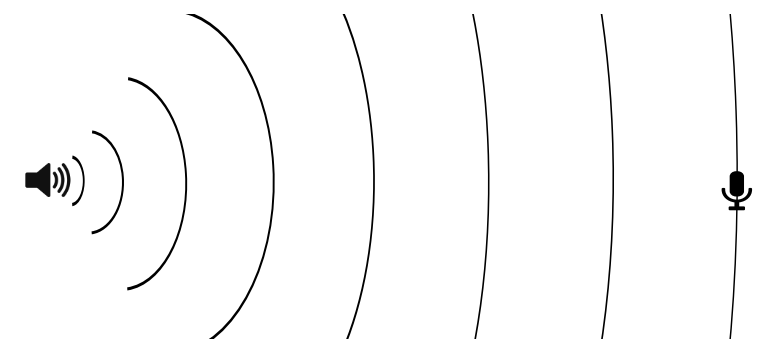
\includegraphics[width=\linewidth]{general/planewaves.png}
    \captionof{figure}{%
    Visualization of the sound propagation. Since the sensor (i.e. a microphone)
    is drawn in the far field, the incoming waves can be approximated as plane waves.
    }
    \label{fig:acoustics:planewaves}
}
When the distance between the source and the receiver is small, typically less than $2\lambda$, the scenario is called \textit{near field}.

\sidenote{Nothing comes from noting. In latin \textit{nihilo nihil fit} ---Parmenide}

%%%%%%%%%%%%%%%%%%%%%%%%%%%%%%%%%%%%%%%%%%%%
\section{Acoustic Reflections}\label{ch:acoustics:sec:reflection}

\todo{From Schimmel's paper, Kutruff and Remaggi}
\todo{Speak about far-field}
% The acoustic reflection are the main object of this thesis.
The equations derived so far assumed unbounded medium, \ie/ free space: a rare scenario in everyday applications.
Real mediums are typically bounded, limited, at least partially.
For instance in a room, the air (propagation medium) is bounded by walls, ceiling, and floor.
When sound travel outdoor, the ground acts as a boundary for one of the propagation direction.
Thus, the sound wave does not just stop when it reaches the end of the medium or when it encounters an obstacle in its path.
Rather, a sound wave will undergo certain behaviors depending on the obstacle acoustics and geometrical properties, including
\begin{itemize}
    \item \textit{reflection} off the obstacle,
    \item \textit{diffraction} around the obstacle,
    \item and \textit{transmission} into the obstacle, causing
    \begin{itemize}
        \item \textit{dissipation}, and
        \item \textit{refraction}.
    \end{itemize}
\end{itemize}

In order, reflections arise typically when a sound wave hit a large surface, like a room wall.
\\Instead, when the sound meets a wall edge or a slit, the wave diffracts, namely it bends around the corners of an obstacle.
The point of diffraction effectively becomes a secondary source which may interact with the first one.
\\The part of energy transmitted to the object may be \textit{absorbed} and \textit{refracted}.
In fact, the object is characterized by a proper acoustic resistance, called \textit{acoustic impedance}, which
describes its acoustic inertia as well as the energy dissipation.
The remaining contribution may continue to propagate causing resulting in the \textit{refraction} phenomenon.
This is more commonly observed when light pass thought different medium, like a prism.

\newthought{When sound reflects}, part of its energy
\begin{itemize}
    \item is reflected \textit{specularly}, \ie/, the angle of incidence equals the angle of reflection; and
    \item is reflected \textit{diffusely} - or \textit{scattered}, \ie/, scatter in every direction).
\end{itemize}


In general, all these phenomena occurs in different proportions depending on the acoustics and geometrical properties of surface as well as
the frequencies content of the wave.
In acoustics, the \textit{operating point} is determined by the sound \textit{wavelength} $[\si{\metre}]$,
\begin{equation}
    \lambda = \frac{2 \pi}{k} = \frac{\speedOfSound}{f}
    ,
\end{equation}
where $f$ is the frequency of the sound wave.
$\lambda$ measures the spatial distance between two molecules in the medium having the same value of pressure
\marginpar{%
a frequency of $\SI{1}{\kHz}$ corresponds to a wavelength of approximately $\SI{34}{\cm}$ ,
which is one or two orders of magnitude smaller than typical linear dimensions of rooms,
as well as typical distances traveled by sound waves in a room
}.
\\Using this quantity we can identify the following three response of the objects (irregularities) of size $d$ to a plane-wave
\begin{itemize}
    \item $\lambda \gg d$, the irregularities are negligible and the sound wave reflection is of specular type;
    \item $\lambda \approx d$, the irregularities break the sound waves which is reflected towards every direction;
    \item $\lambda \ll d$, each irregularities is a surface reflecting specularly the sound waves.
\end{itemize}

% All these effects contributes to create a rich
% It is interesting to note that the diffraction waves produced by the semi-infinite reflector edge allow the area that is “behind” the reflector (i.e. the so called shadow zone), to be reached by the propagating sound.

\newthoughtpar{In the previous section,} we manipulated the wave equation in free space.
However in case of modeling reflection for indoor propagation, working with those formulas might results complicated and difficult.
A simplified yet effective approach is to model incoming sound waves as \textit{acoustic rays}, namely
a small portion of a the wave emitted by a point source in a room.
This ray has well-defined direction and velocity of propagation, and conveys a total energy which remains constant.
This simplified description undergoes with the name of \textit{geometrical acoustics} (GA), and share many fundamentals with geometrical optics.

This model will be convenient to describe and visualize the reflection behavior hereafter.

\subsection{Large smooth surfaces, absorption and echoes}
\todo{Savioja2015geometric}
% The main focus of this section and the this whole thesis goes on \textit{specular reflections}.
Specular reflection occurs when sound bounces off surfaces which can be modelled as infinite flat and smooth surfaces.
This happens when the surface has dimension much bigger than the sound wavelength and it results in a mirror-like effects.
Here the acoustic ray is reflected according to the \textit{law of reflection}, stating that
(i) the reflected ray remains in the plane identified by the incident ray and the normal to the surface,
and (ii) the angles of the incident and reflected rays with the normal are equal.
\marginpar{%
    \centering
    \footnotesize
    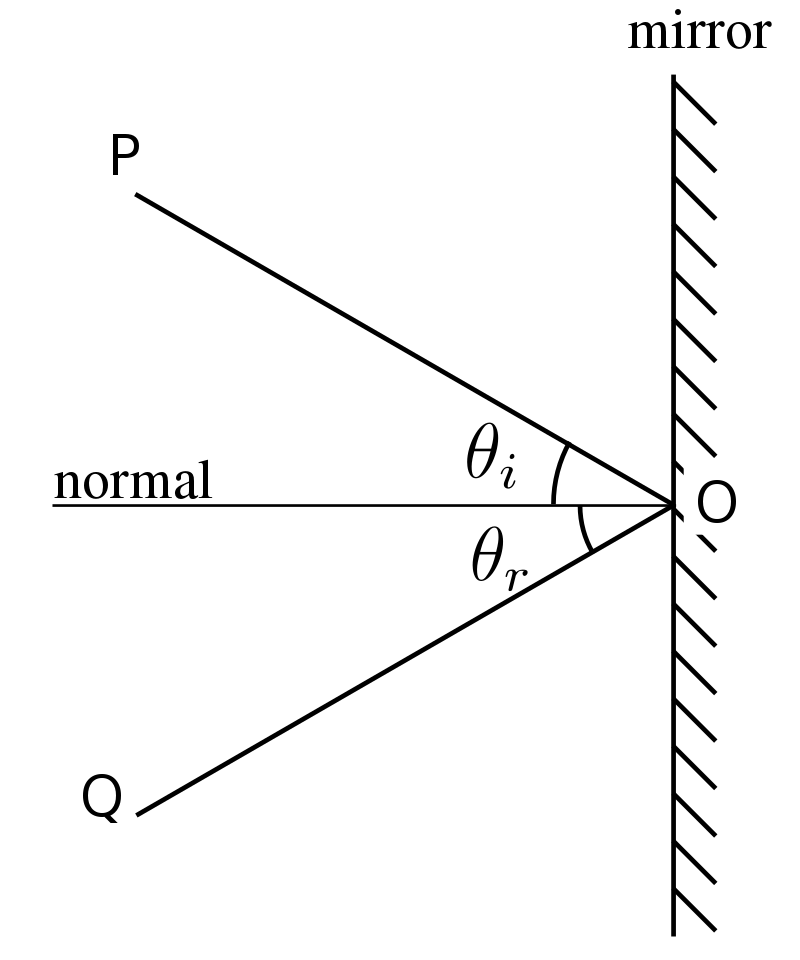
\includegraphics[width=\linewidth]{general/reflection_law.png}
    \captionof{figure}{%
        Specular reflection
    }
    \label{fig:mirage:scene}
}

\newthoughtpar{Absorption (and Reflection) coefficient}
The proportion of energy absorbed by the surface and the incident acoustic wave is measured
through the reflector's \textit{acoustic impedance}\sidenote{%
\textbf{acoustic impendence} measures the opposition that an acoustic system presents to the acoustic pressure.
}.
By relating the acoustic pressure at the reflector location with the velocity of the incoming plane waves,
one can derive the \textit{plane-wave reflection coefficient} or \textit{pressure reflector factor} $\reflCoeff$ \cite{kuttruff} as
\begin{equation}
    \reflCoeff(f, \theta) = \frac{\impedence_w(f)\cos(\theta) - \impedenceAir(f)}{\impedence_w(f)\cos(\theta) + \impedenceAir(f)}
    ,
\end{equation}
where $\impedence_w(f)$ and $\impedenceAir(f)$ are the frequency-dependent impedance of the surface and the air respectively,
and $\theta$ is the angle of incidence.

This formula holds as long as the far field assumption is verified as well for the reflectors:
the source, or receiver, is several wavelengths away from the infinite reflecting plane.

Within the context of \GA/, it is common to use consider the energy or the intensity of the plane wave, which is
proportional to the square of the pressure amplitude. Thus, it is customary to use the absorption coefficient,
\begin{equation}
    \absCoeff = 1 - \abs{\reflCoeff(f, \theta)}^2
    ,
\end{equation}
where the phase information of the reflection process is lost.
\\Estimating acoustic impedance and absorption coefficient of a real material and difference between them has long been a topic of study
In audio signal processing and in acoustics,

However, data made available by surface material manufacturers is typically measured according to the reverberation room standard, with octave-band or third-octave-band reso- lution for the range 100 Hz–5 kHz,
true arand has long been a topic of study

Moreover, the dependency on the angle is often relaxed in favor of a more simplified yet solid parameter where
averaged across incidence angles h is the quantity that is used by various implementations of the GA techniques.

Specular reflection results in a delta-like peak in the function such that all of the energy is reflected in one direction, while the function takes on a value of 0 elsewhere

\subsection{Diffusion, Scattering and Diffraction}
Real-world surfaces are not ideally flat and smooth; they may includes various irregularities.
Examples of such surfaces are coffered ceilings, faceted walls, raw brick walls as well as the entire audience area of a concert hall.
When the \textit{roughness} of the surface is in the same order of the sound wavelength, \textit{diffuse reflection} is observed.
% \cite{Dalenback1994macroscopic}

The acoustic ray can be thought of as a bundle of individual rays which are traveling parallel.
When it strikes the surface, each individual rays are bounced off irregularly, creating \textit{scattering}.
In the context of \GA/, this type of reflection is modeled as a number of new rays, uniformly distributed in the original half-space.
The total amount of energy of this reflection may be computed a-priori with the surface \textit{scattering} coefficient
or a-posteriori with the \textit{diffuse coefficient}, namely the ratio between
the specularly reflected energy over the total reflected energy.

This process is well modeled thought the \textit{Lambert's emission law}, which was original used to describe optical diffuse reflection.

\newthought{Diffraction} occurs at the boundaries of semi-finite surfaces, for instance around corners or through door openings.
to be continued...


% -----------------------------------------------------------------------------

\section{Room Acoustics and Room Impulse Response}\label{ch:acoustics:sec:rir}
Room acoustics concerns with acoustic waves propagating in air enclosed in a volumes with a set of surfaces
(walls, floors, etc.), from which an incident wave may be interact as described in \cref{ch:acoustics:sec:reflection}.
Thus, a room is a physical enclosure that containing the medium and has boundaries that limit the sound propagation.

% By adding boundary condition we can now write the wave equation for indoor propagation, namely within a 3-dimensional enclosure.
% Let us assume the simplest possible 3-D enclosure: a cuboid room with perfectly smooth and rigid facets
% \sidenote{%
% \textbf{facet}: each of the plane surfaces of a polytope.
% }.
% More precisely, let define $\calC$ the domain of the problem as the cuboid with length $L$, width $W$ and height $H$, that is
% \begin{equation}
%     \calC = \kset{\positionMicrophone = (x,y,z)}{
%         0 \le x \le L,\,
%         0 \le y \le W,\,
%         0 \le z \le Z}
% \end{equation}
% Let $\calB$ be the boundaries of $\calC$, \ie/ the rigid room facets.

Given the boundaries $\calB$, the frequency-domain Green's function associated to \cref{eq:acoustics:helmholtz} is given by
\begin{equation}
    \label{eq:acoustics:greenBounded}
    H(f, \positionMicrophone \mid \positionSource) =
        - \frac{1}{V}
        \sum_{\pos=-\infty}^{\infty}
        \frac{\Psi_{\pos}(\positionMicrophone)\Psi_{\pos}(\positionSource)}{\kappa_{\pos} - \kparen{\sfrac{f}{c}}^2}
\end{equation}
where
\begin{equation}
    \psi_{\pos}(\positionMicrophone) =
\end{equation}
is the eigenfunction for the boundaries $\calC$.

The inverse Fourier transform of the frequency response of the room described by (13)leads to a RIR,h(r,rs,t).

\newthought{Mathematically the sound propagation} is described by the wave equation.
An impulse response from a source to a microphone can be obtained by solving the wave equation.
Since it can seldom be expressed in an analytic form the solution must be approximated.


\subsection{the Image Model and the Image Method}
Finally, the equation becomes
\begin{equation}
    \label{eq:acoustics:ims:frourier}
    H(f, \positionMicrophone \mid \positionSource) =
        \sum_{p=1}^{8}
            \sum_{\pos=-\infty}^{\infty}
                \frac{1}{4 \pi \norm{\coordinatePermutation_p +  \coordinatePermutation_p}}
\end{equation}

by taking the inverse Fourier Transform, the echo structure becomes explicit.

https://reuk.github.io/wayverb/context.html

We can write the final Room Impulse Response $\rir_{ij}(t)$ as follows:
\begin{equation}
    \contMicrophoneSignal(t) = (\rir_{ij} \conv \contSource)(t)
\end{equation}

\begin{equation}
    \rir_{ij}(t) = \sum_{r=0}^{R} \frac{\alpha_r}{4 \pi \tau_r / \cair} \delta \kparen{t - \tau_r}
\end{equation}
where
\begin{itemize}
    \item $\alpha_r \in \kintervcc{0}{1}$ is the attenuation coefficient of the $r$-th reflection
    \item $\tau_r = \norm{\positionMicrophone_\idxMic - \positionSource_\idxEch}$ is the distance between the microphone and the $\idxEch$-th image of source $\idxSrc$.
\end{itemize}

\subsection{Simulating Room Acoustics}
Sound propagation is well described mathematically by the wave equation.
By solving it, the Room Impulse Response can be obtained.
however its analytic solution is a cumbersome task, thus its solution must be approximated: it can be found only in extrimely
simple cases such as a 3D shoebox.
There are two main categories: geometric and wave-based~\cite{Habets2010generator, reuk.github.io, Savioja2015goemetric}.
\begin{itemize}
    \item \textit{wave-based} aims at solving wave equation numerically, while
    \item \textit{geometric} methods make some simplifying assumption about the wave propagation. It results a less accurate, but faster simulation.
    They assumption typically ignore the \textit{wave} behavior of the sound, choosing much lighter model such as \textit{ray}s or \texit{particle}s.
\end{itemize}

\newthought{Wave-based}. Most accurate, but computationally more demanding.

% description
the Element methods:
\FEMf/ divide the space into small volume elements smaller of the sound wavelengths,
\BEMf/ divide only the boundaries of the space are divided into surface elements.
This elements interact with each other according to the math of the wave equation.
At high frequencies, the elements must be very small, so their number increases, so the computational complexity increases.
This are better for low frequencies and small enclosures.
\FDTD/ methods replacing the derivatives in the wave equation, with its discrete approximation, \ie/ finite differences.
\DWM/ methods..

% drawbacks
For the wave-based method the most difficult part is the definition of the boundaries condition.
Their require for instance to know the complex impedances of the surfaces, a parameter hard to find in the literature.

% modes
On the other hand, these methods inherently account for effects such as diffraction and interference.
This methods are capable of simulating the low-frequencies components of the \RIR/, where they contribute form \textit{room modes}.
Modes have the effect of amplifying and attenuating specific frequencies in the \RIR/, and produce much of the subjective sonic “colour” or “character” of a room.
Reproducing this modes is of vital importance for evaluating acoustic of rooms, such as concert hall, and recording studios or when producing musically pleasing reverbs.



\newthought{Ray-tracing}. Modeling of waves as discrete particles Great success in the field of computer graphics for modeling reflection of light.
The assumption that rays and waves are interchangeable is good for high frequencies. For low frequencies, where the wavelength are of the same order
of the wall surface, it may leads to strong approximation error: interferences and diffractions effects are not taken into account at these frequencies\cite{Savioja2015goemetric}.


\newthought{Hybrid Methods}

\subsection{The Acoustic Impulse Response}
The multiple sound propagation paths from a source to a receiver in a room can be
modeled accurately by a linear time-invariant system defined by the so-called room impulse response.
A room impulse response contains several perceptually relevant components


\subsection{Properties of the Room Impulse Response}
\newthoughtpar{direct path}
\newthoughtpar{early echoes}
\newthought{The echoes are} specular reflections which stand out in terms of strength or timing.
Whether a reflection will become an echo or not depends on its delay with respect to the direct sound, on its relative strength, on the nature of the sound signal, and on the presence of other reflections which eventually mask the reflection under consideration
the term ‘echo’ will be used for any sound reflection which
is subjectively noticeable as a temporal or spatially separated repetition of the original sound signal, and we are discussing the conditions under which a reflection will become an echo
\newthoughtpar{Echoes}
The \textit{echoes} are a particular type of specular reflection.
Whether a reflection can be defined as a echo or not depends
on the delay with respect to the direct sound and its relative strength.
Originally, echo referred to

\marginpar{%
    The word echo derives from the Greek
    %ἠχώ (ēchō),[1] itself from ἦχος (ēchos), "sound".[2]
    Echo in the folk story of Greek is a mountain nymph whose ability to speak was cursed,
    only able to repeat the last words anyone spoke to her.
}
% In the following the term ‘echo’ will be used for any sound reflection which
% is subjectively noticeable as a temporal or spatially separated repetition of the original sound signal, and we are discussing the conditions under which a reflection will become an echo. Thus we are taking up again the second question raised at the outset of the foregoing section.

\newthoughtpar{late reverberation}

\subsection{Room Acoustic Simulators}
https://reuk.github.io/wayverb/context.html

%%%%%%%%%%%%%%%%%%%%%%%%%%%%%%%%%%%%%%%%%%%%
\section{Acoustic Parameters and Perception}
\itodo{cite Sacks}
\newthoughtpar{The Mixing Time}
\newthoughtpar{Reverberation Time}
\newthoughtpar{Direct-to-revebrerant ratio}
\newthoughtpar{Critical Distance}
\newthoughtpar{Interchannel Coherence}
\newthoughtpar{Perception of the Early Reflection}
At low levels it manifests itself only by an increase of loudness of the total sound signal, by a change in timbre, or by an increase of the apparent size of the sound source. But at higher levels a reflection can be heard as a separate event, i.e. as a repetition of the original sound signal
\newthoughtpar{Perception of the Late Reverberation}